\section{Appendix}\label{section:appendix}

% ---------------- Part A ----------------
\begin{figure}[H]
    \centering
    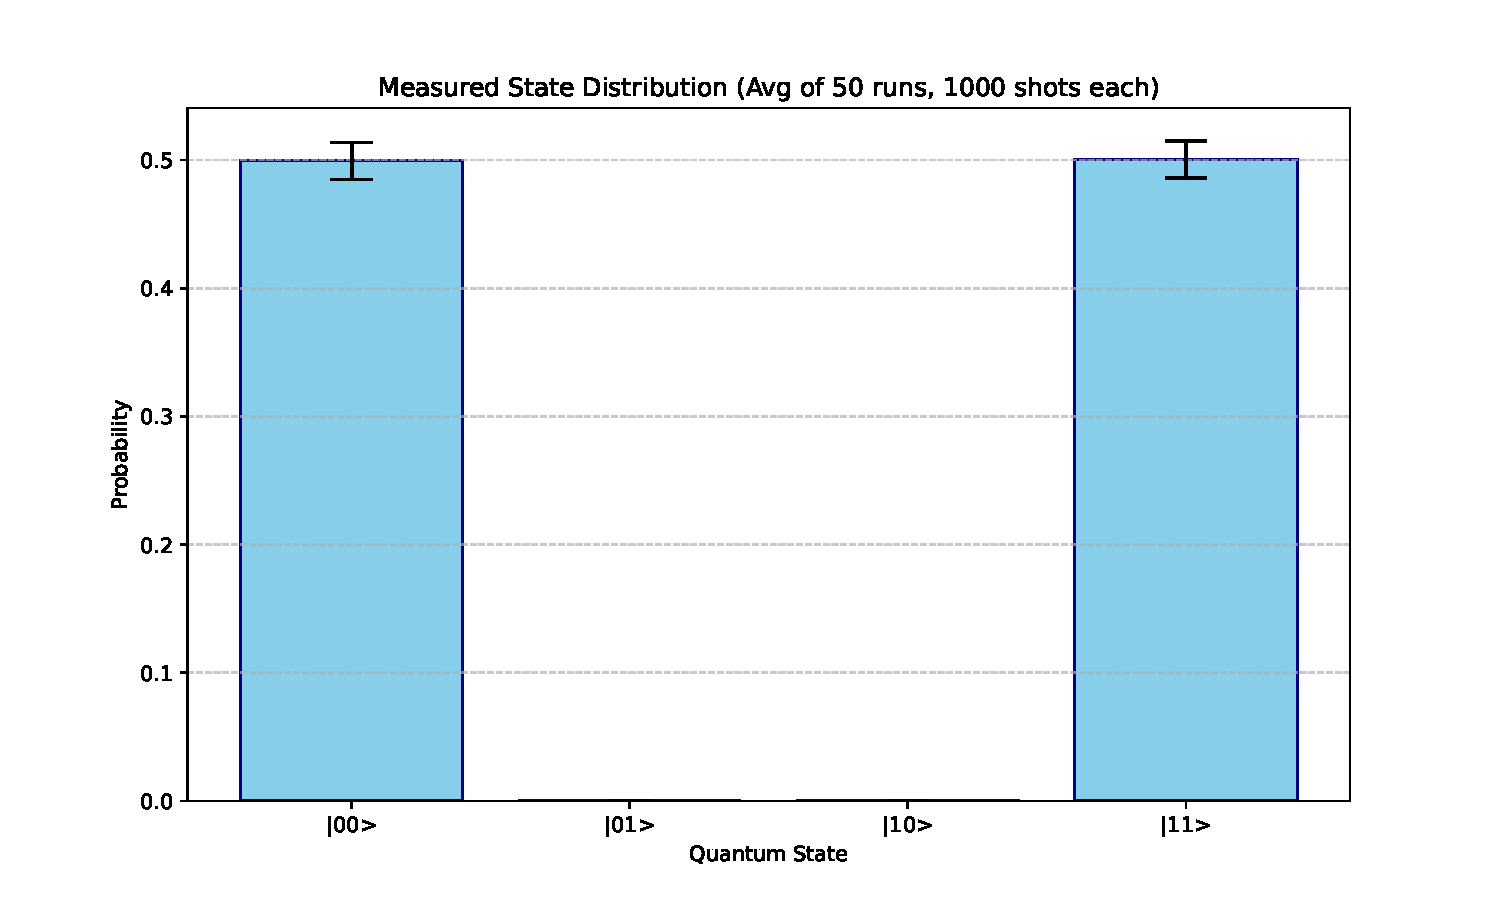
\includegraphics[width=0.55\linewidth]{figures/part-a_measurement_dist.pdf}
    \caption{Measurement distribution (Part A).}
    \label{fig:parta_measurement_distribution}
\end{figure}

% ---------------- Part B ----------------
\begin{figure}[H]
    \centering
    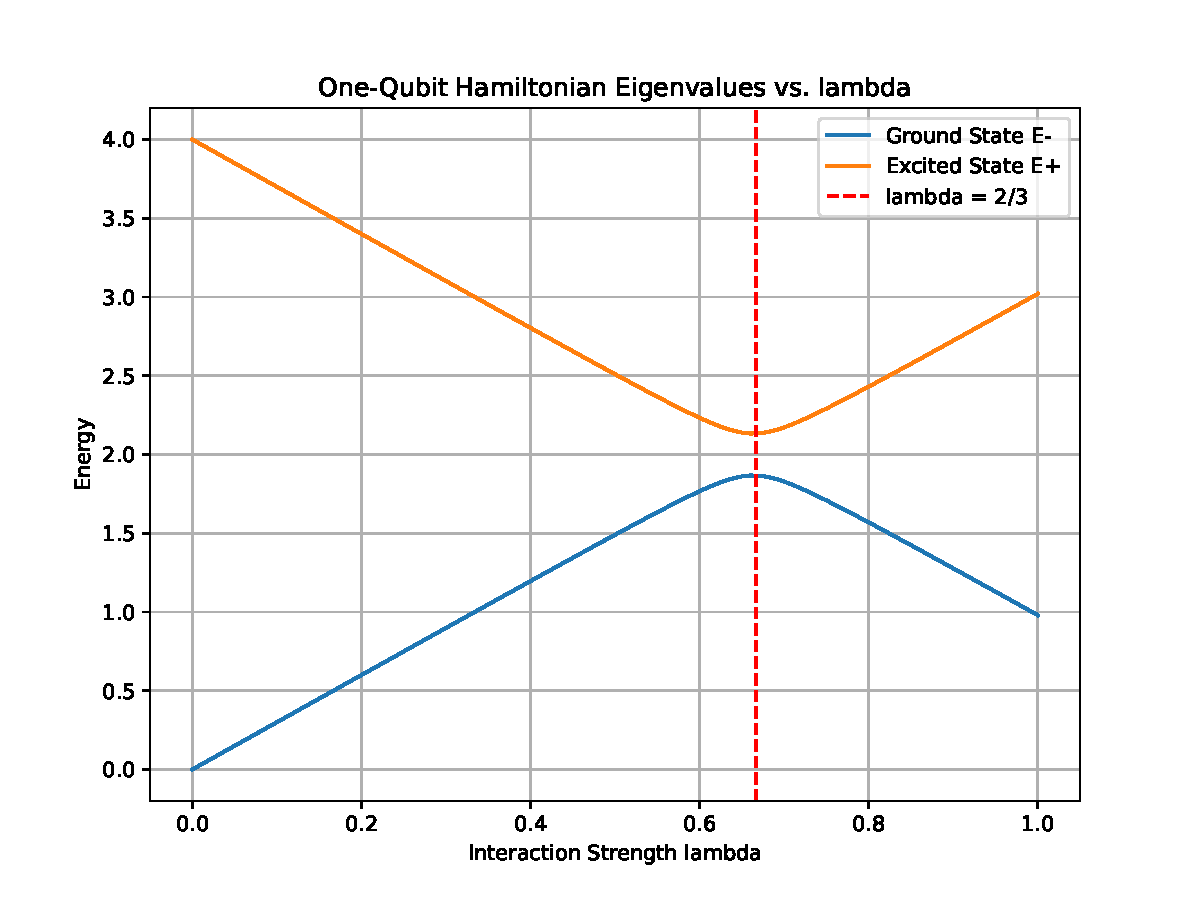
\includegraphics[width=0.55\linewidth]{figures/part-b_eigenvalues.pdf}
    \caption{Eigenvalue spectrum of the Hamiltonian (Part B).}
    \label{fig:partb_eigenvalues}
\end{figure}

\begin{figure}[H]
    \centering
    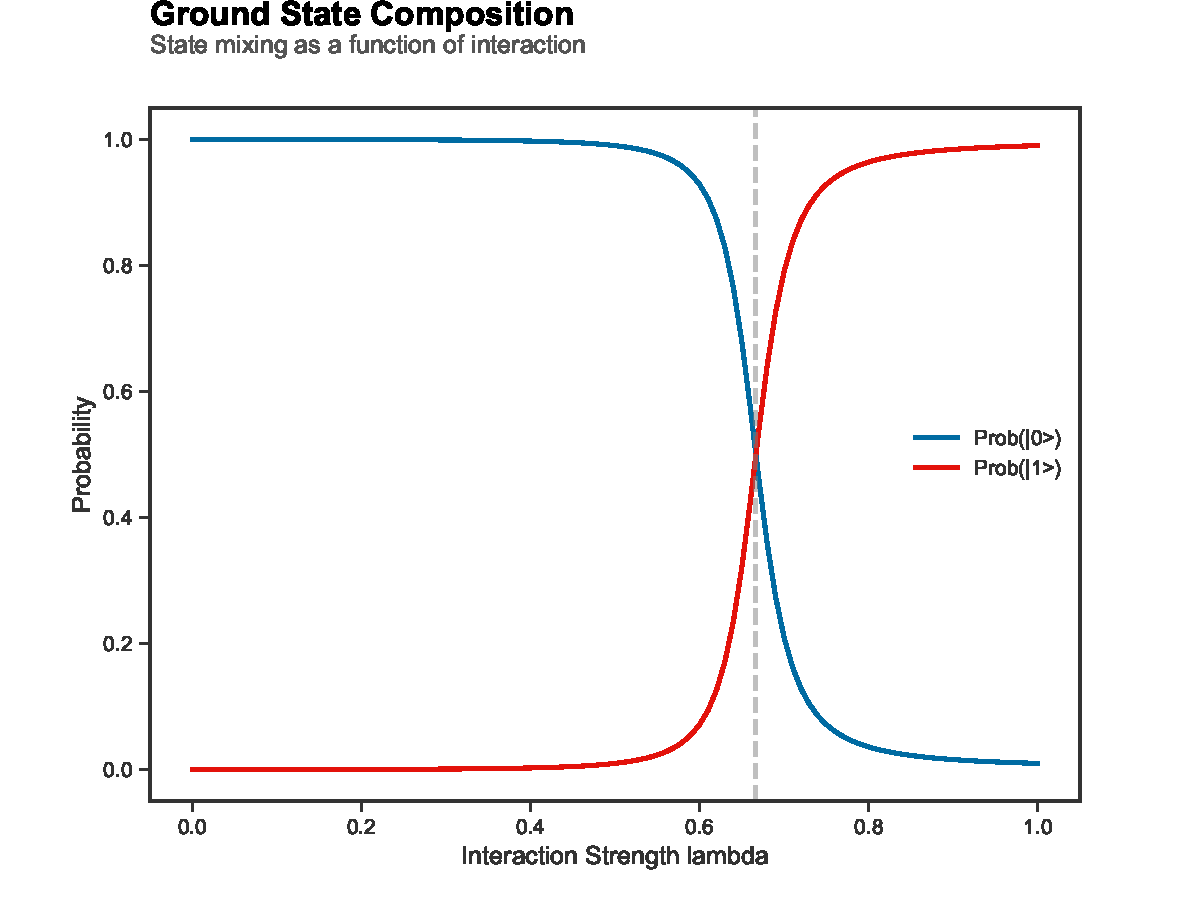
\includegraphics[width=0.55\linewidth]{figures/part-b_eigenvector_mixing.pdf}
    \caption{Eigenvector mixing across the spectrum (Part B).}
    \label{fig:partb_eigenvector_mixing}
\end{figure}

% ---------------- Part C ----------------
\begin{figure}[H]
    \centering
    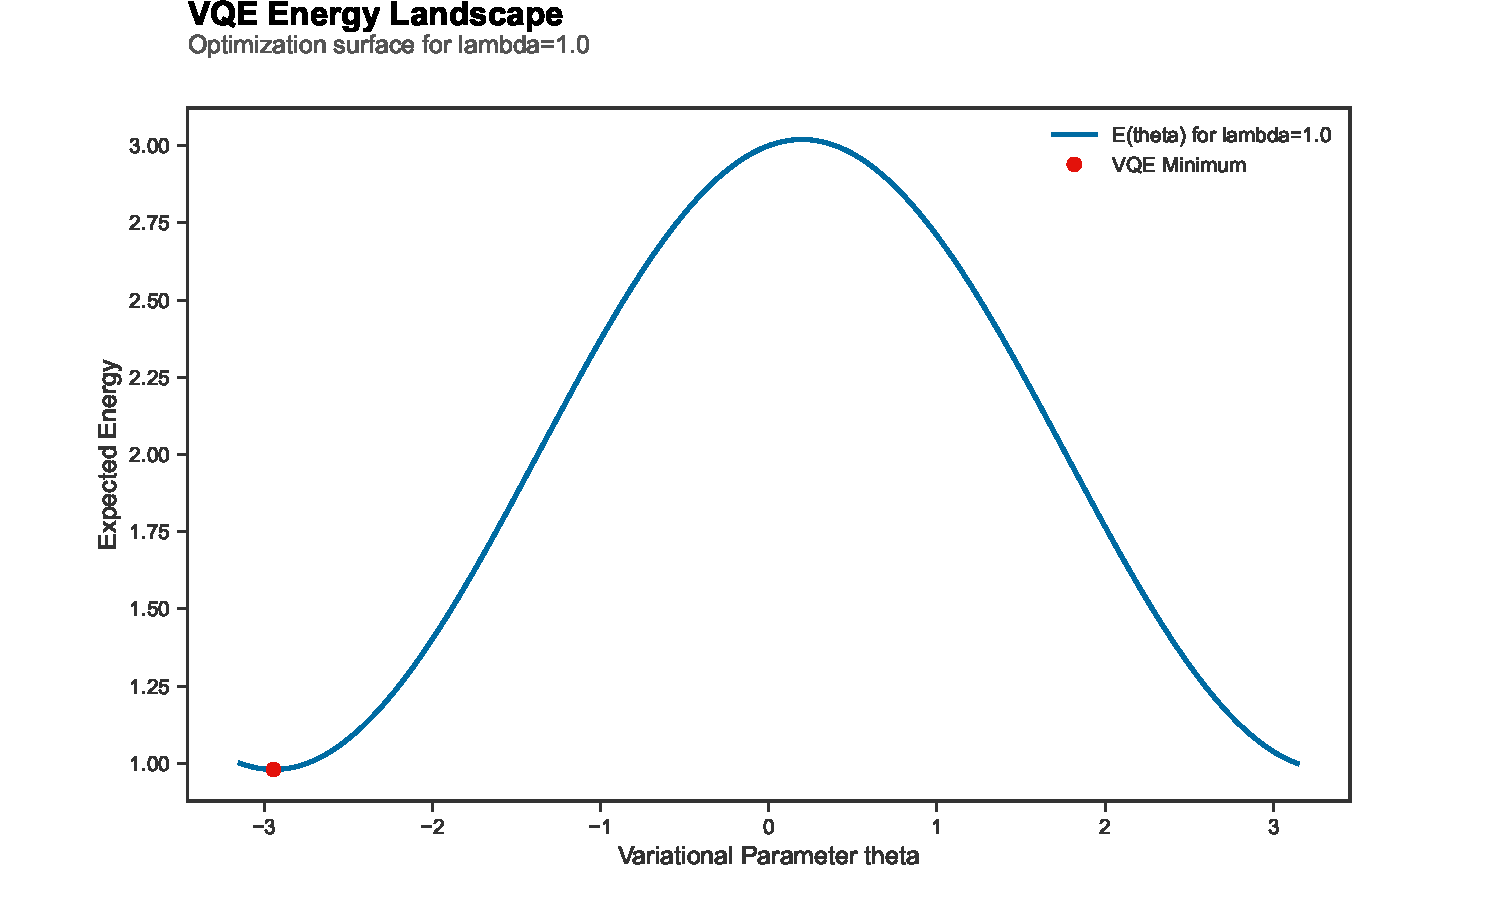
\includegraphics[width=0.55\linewidth]{figures/part-c_energy_landscape.pdf}
    \caption{Energy landscape over the variational parameter space (Part C).}
    \label{fig:partc_energy_landscape}
\end{figure}

\begin{figure}[H]
    \centering
    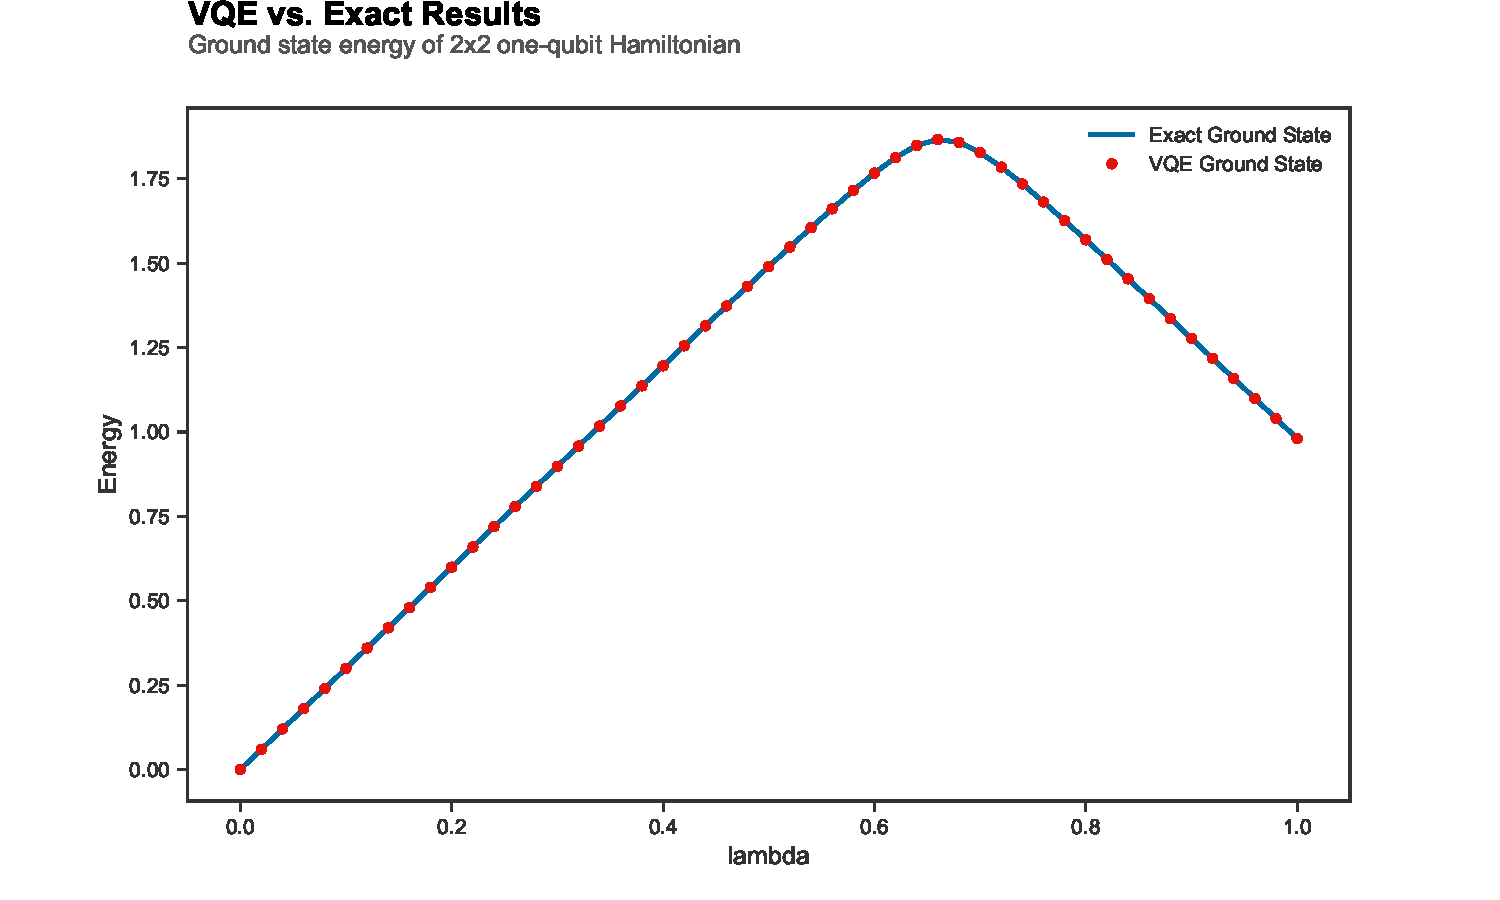
\includegraphics[width=0.55\linewidth]{figures/part-c_vqe_comp.pdf}
    \caption{VQE energy convergence compared to the exact ground-state energy (Part C).}
    \label{fig:partc_vqe_comparison}
\end{figure}

\begin{figure}[H]
    \centering
    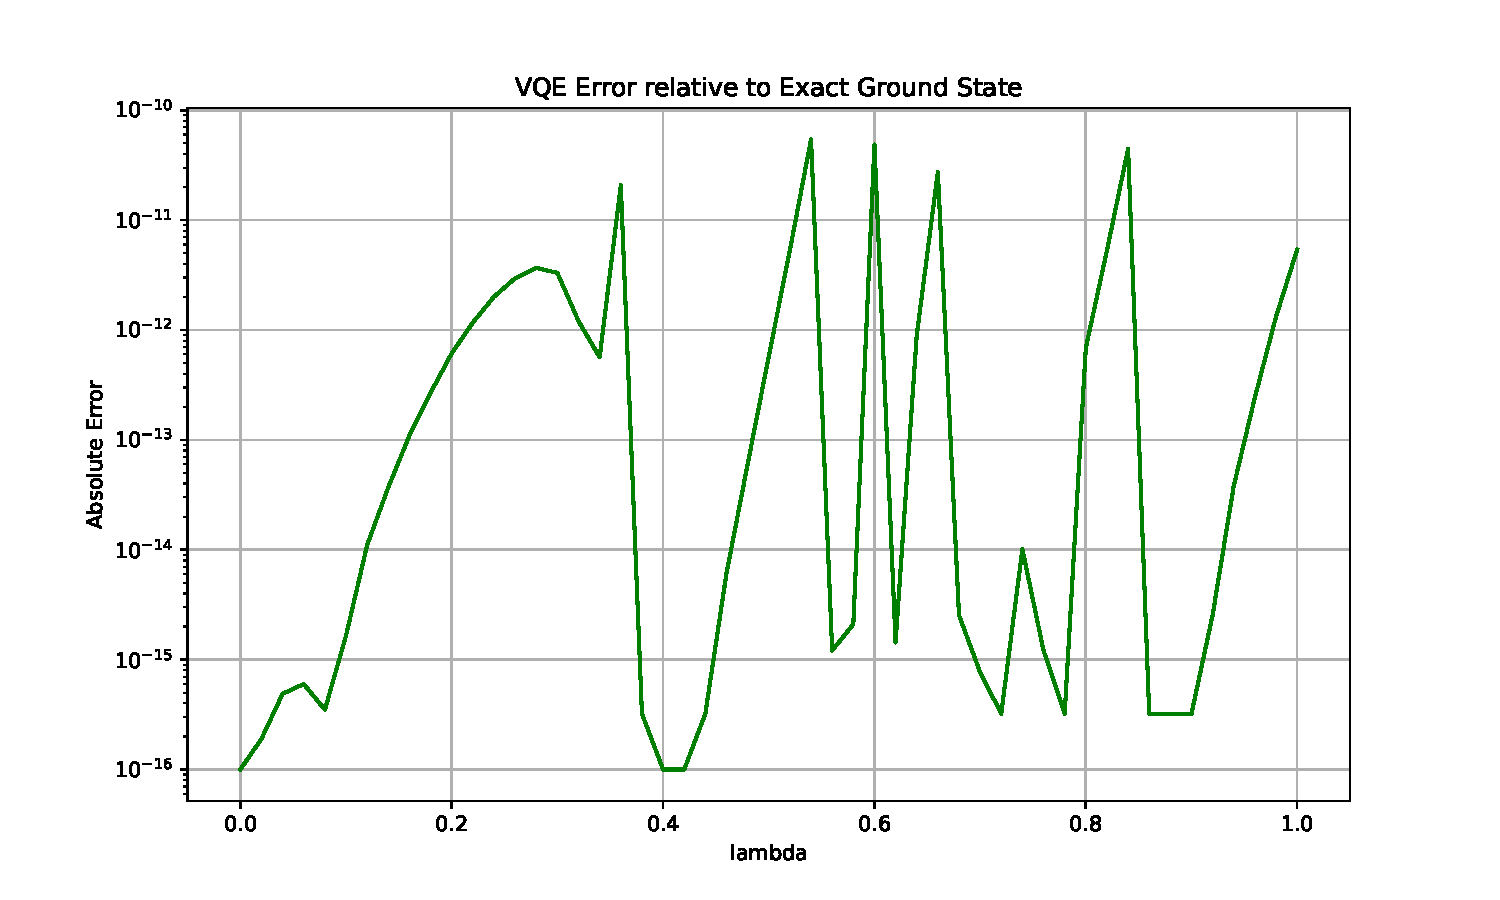
\includegraphics[width=0.55\linewidth]{figures/part-c_vqe_error.pdf}
    \caption{Absolute VQE error as a function of optimization iterations (Part C).}
    \label{fig:partc_vqe_error}
\end{figure}

% ---------------- Part D ----------------
\begin{figure}[H]
    \centering
    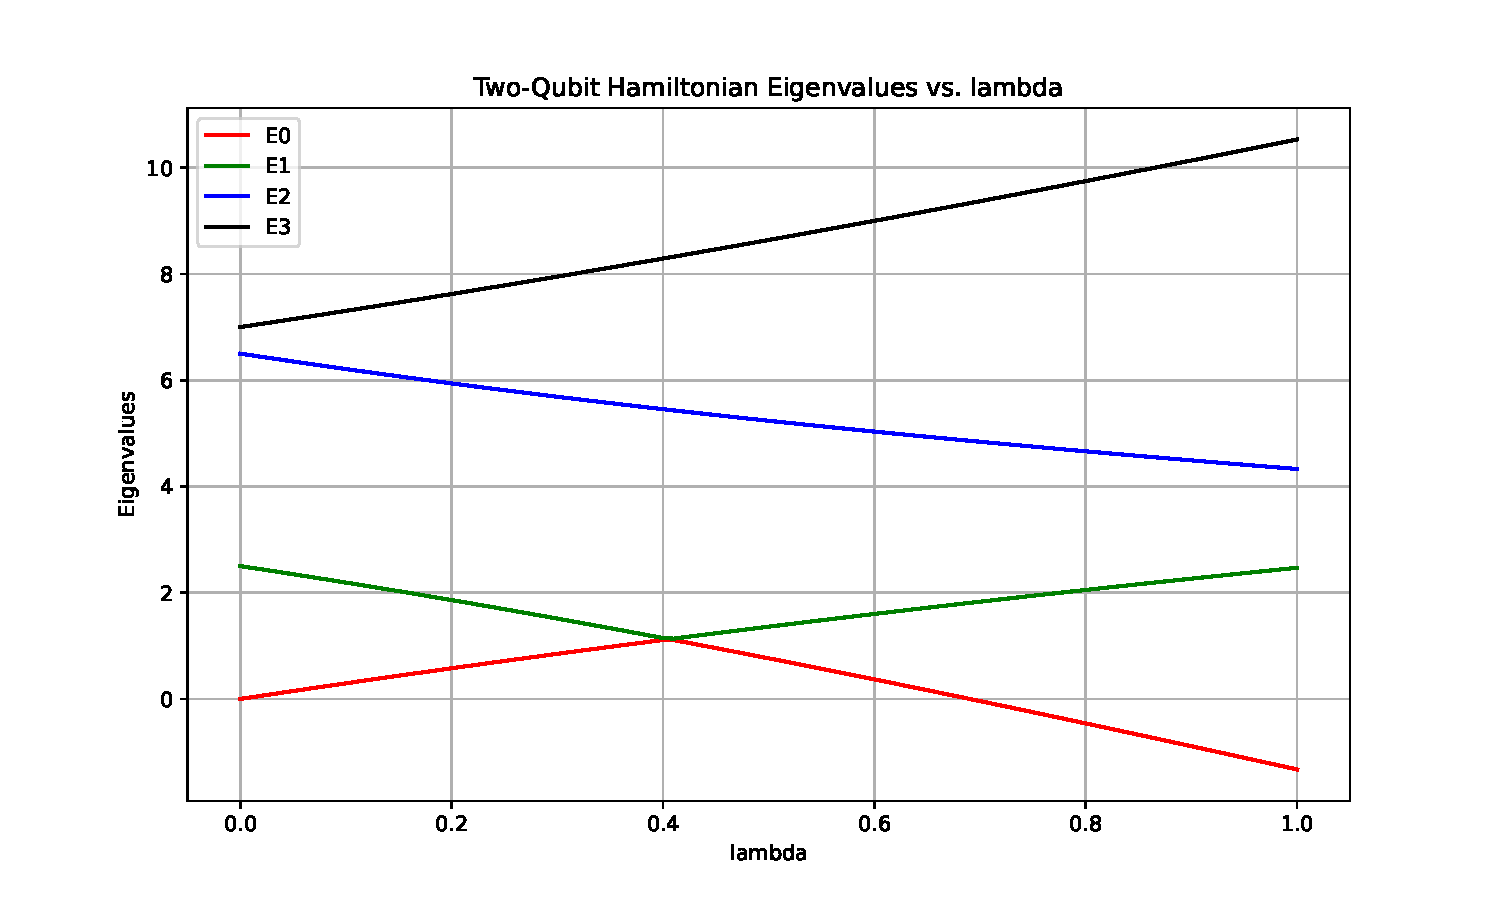
\includegraphics[width=0.55\linewidth]{figures/part-d_eigenvalues.pdf}
    \caption{Eigenvalue spectrum of the extended system (Part D).}
    \label{fig:partd_eigenvalues}
\end{figure}

\begin{figure}[H]
    \centering
    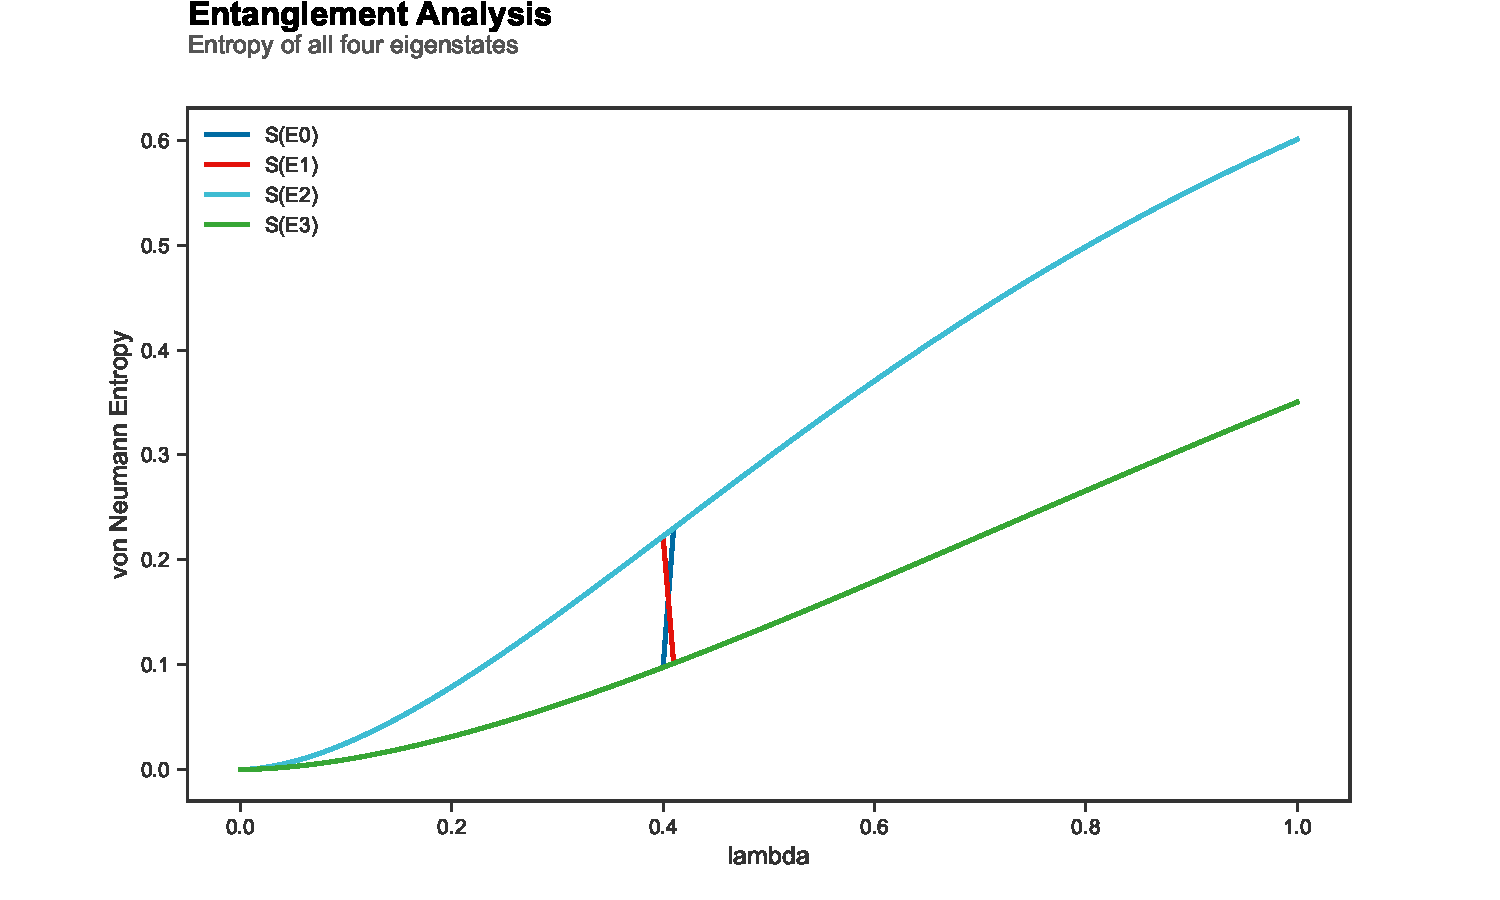
\includegraphics[width=0.55\linewidth]{figures/part-d_entropy.pdf}
    \caption{Bipartite entanglement entropy across system partitions (Part D).}
    \label{fig:partd_entropy}
\end{figure}

% ---------------- Part E ----------------
\begin{figure}[H]
    \centering
    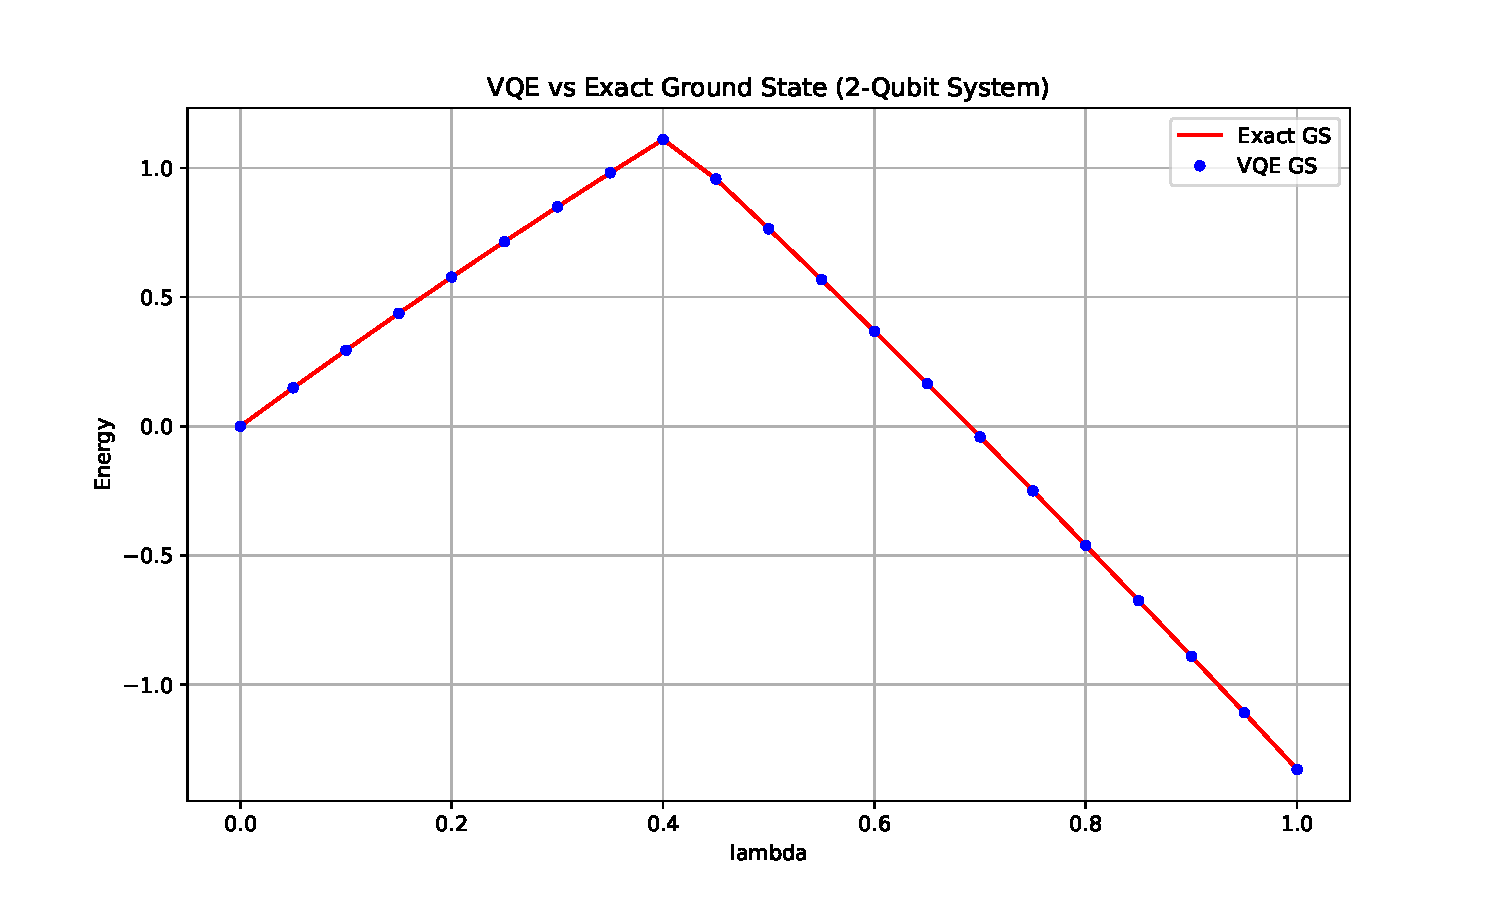
\includegraphics[width=0.55\linewidth]{figures/part-e_vqe_comp.pdf}
    \caption{VQE energy convergence for the modified Hamiltonian (Part E).}
    \label{fig:parte_vqe}
\end{figure}

% ---------------- Part F ----------------
\begin{figure}[H]
    \centering
    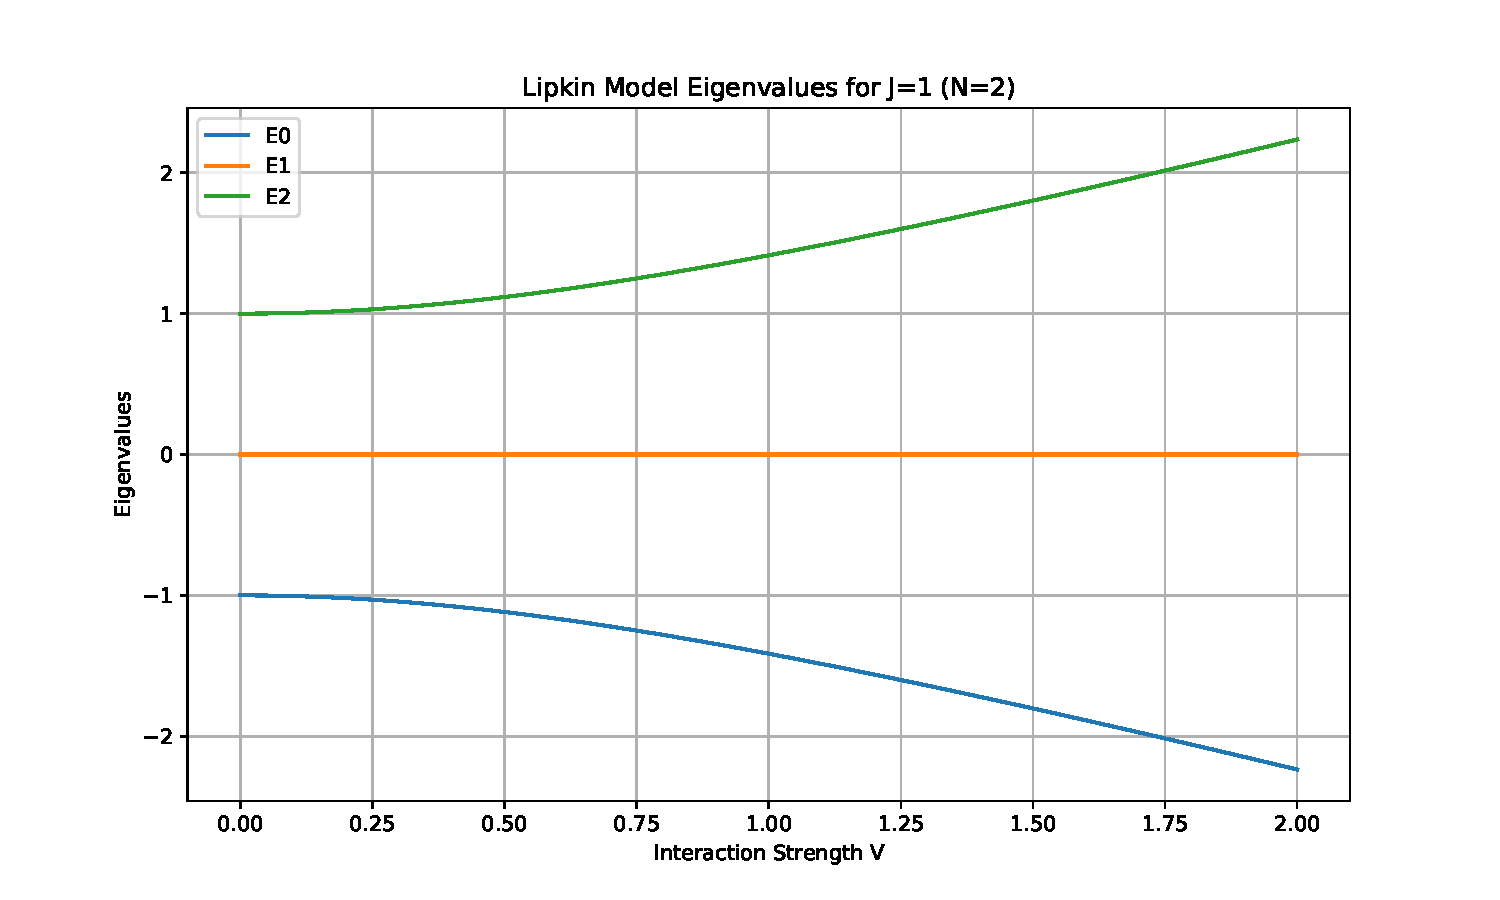
\includegraphics[width=0.55\linewidth]{figures/part-f_j1.pdf}
    \caption{Ground-state energy as a function of coupling parameter $J_1$ (Part F).}
    \label{fig:partf_j1}
\end{figure}

\begin{figure}[H]
    \centering
    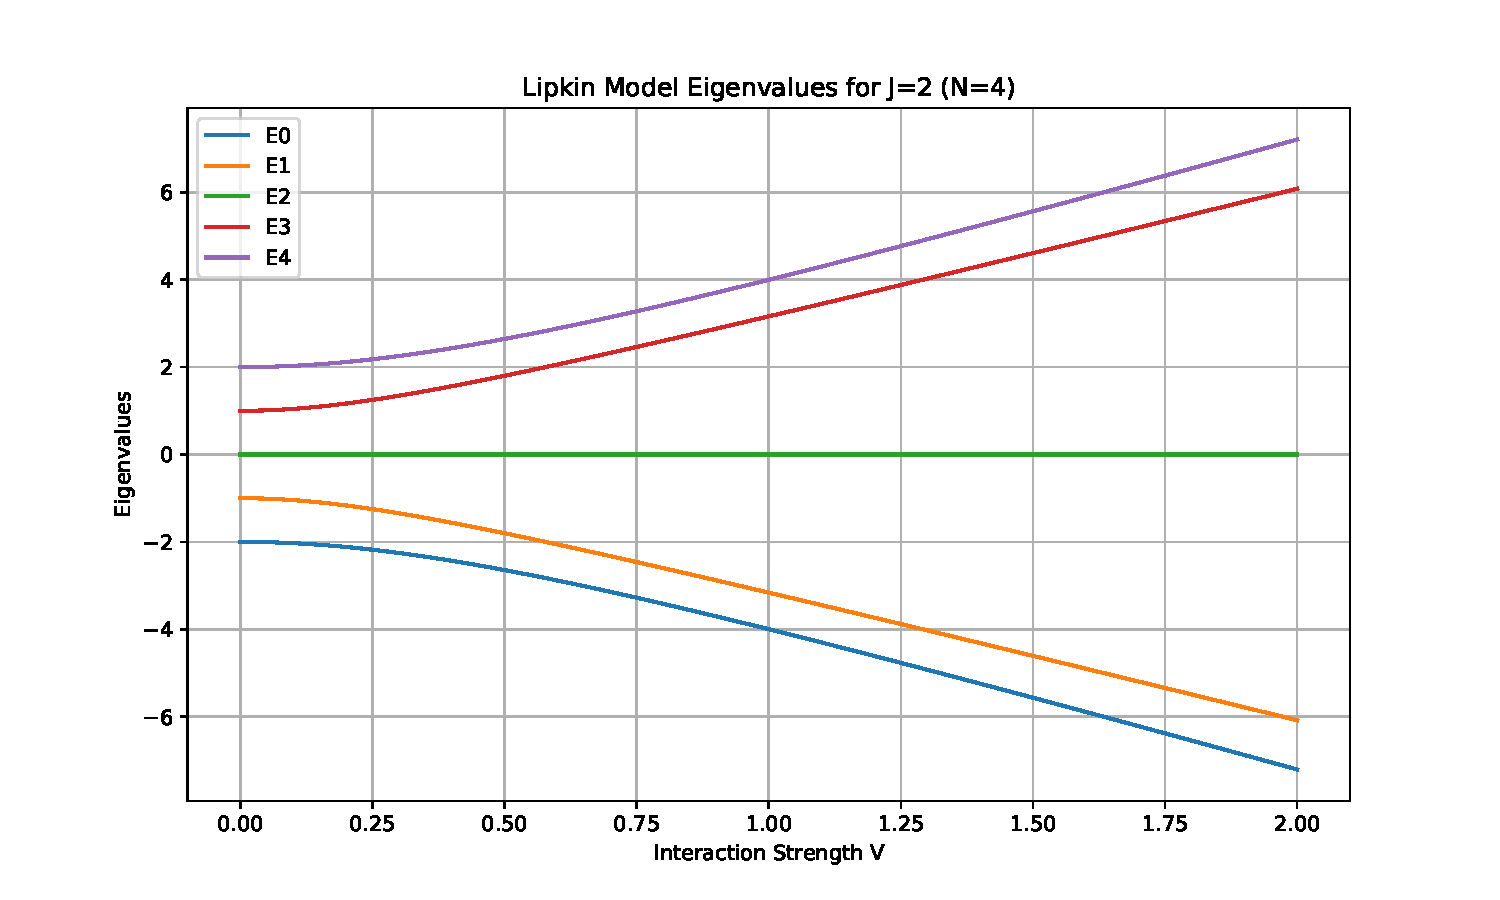
\includegraphics[width=0.55\linewidth]{figures/part-f_j2.pdf}
    \caption{Ground-state energy as a function of coupling parameter $J_2$ (Part F).}
    \label{fig:partf_j2}
\end{figure}

\begin{figure}[H]
    \centering
    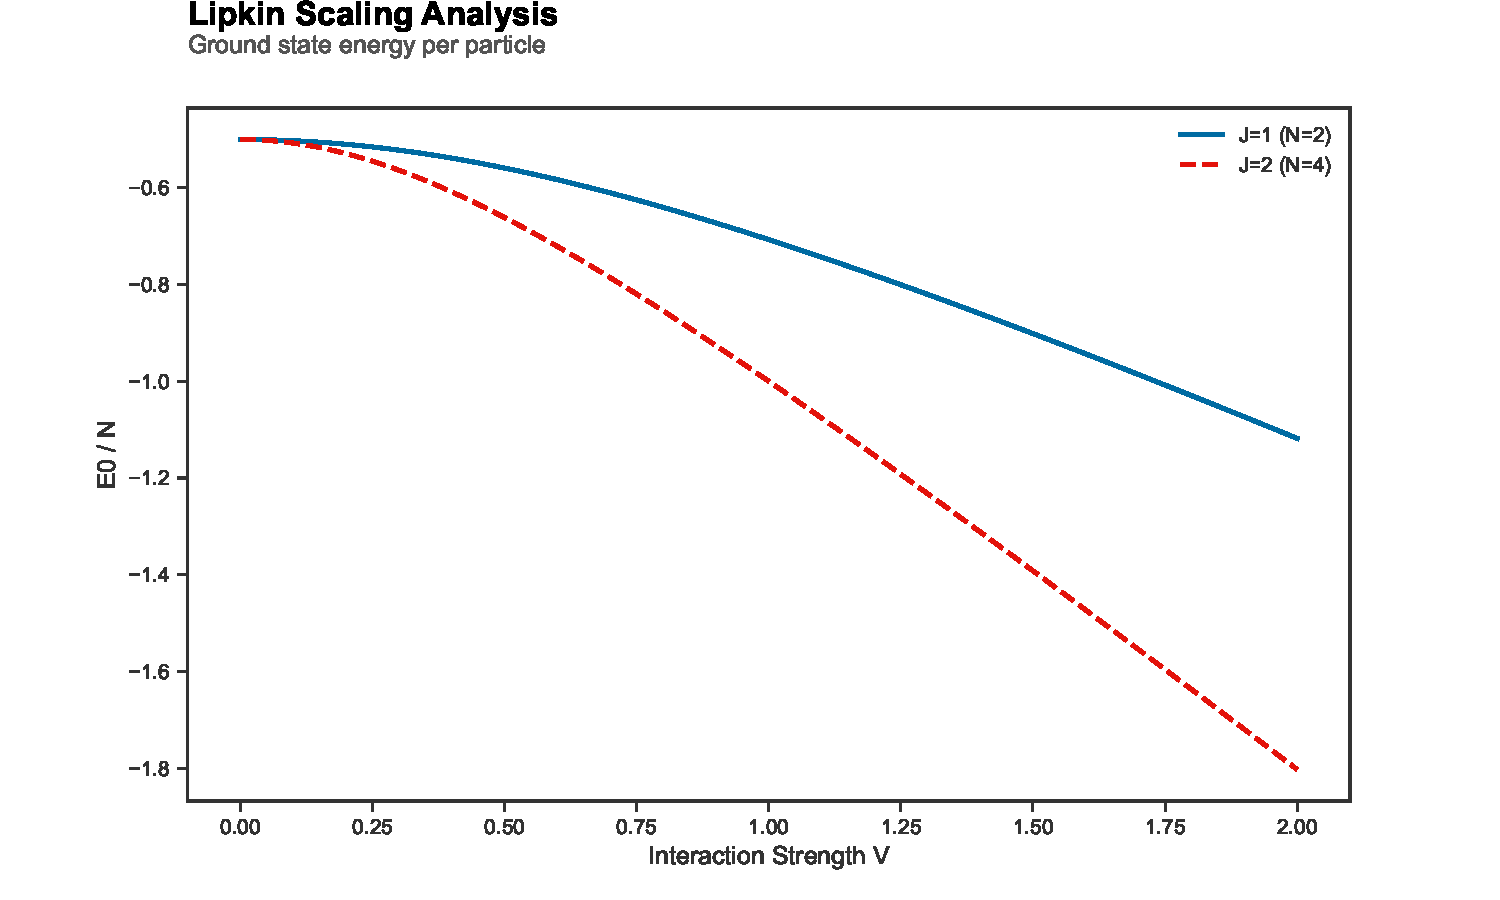
\includegraphics[width=0.55\linewidth]{figures/part-f_scaling.pdf}
    \caption{Scaling behavior of the ground-state energy with system size (Part F).}
    \label{fig:partf_scaling}
\end{figure}

% ---------------- Part G ----------------
\begin{figure}[H]
    \centering
    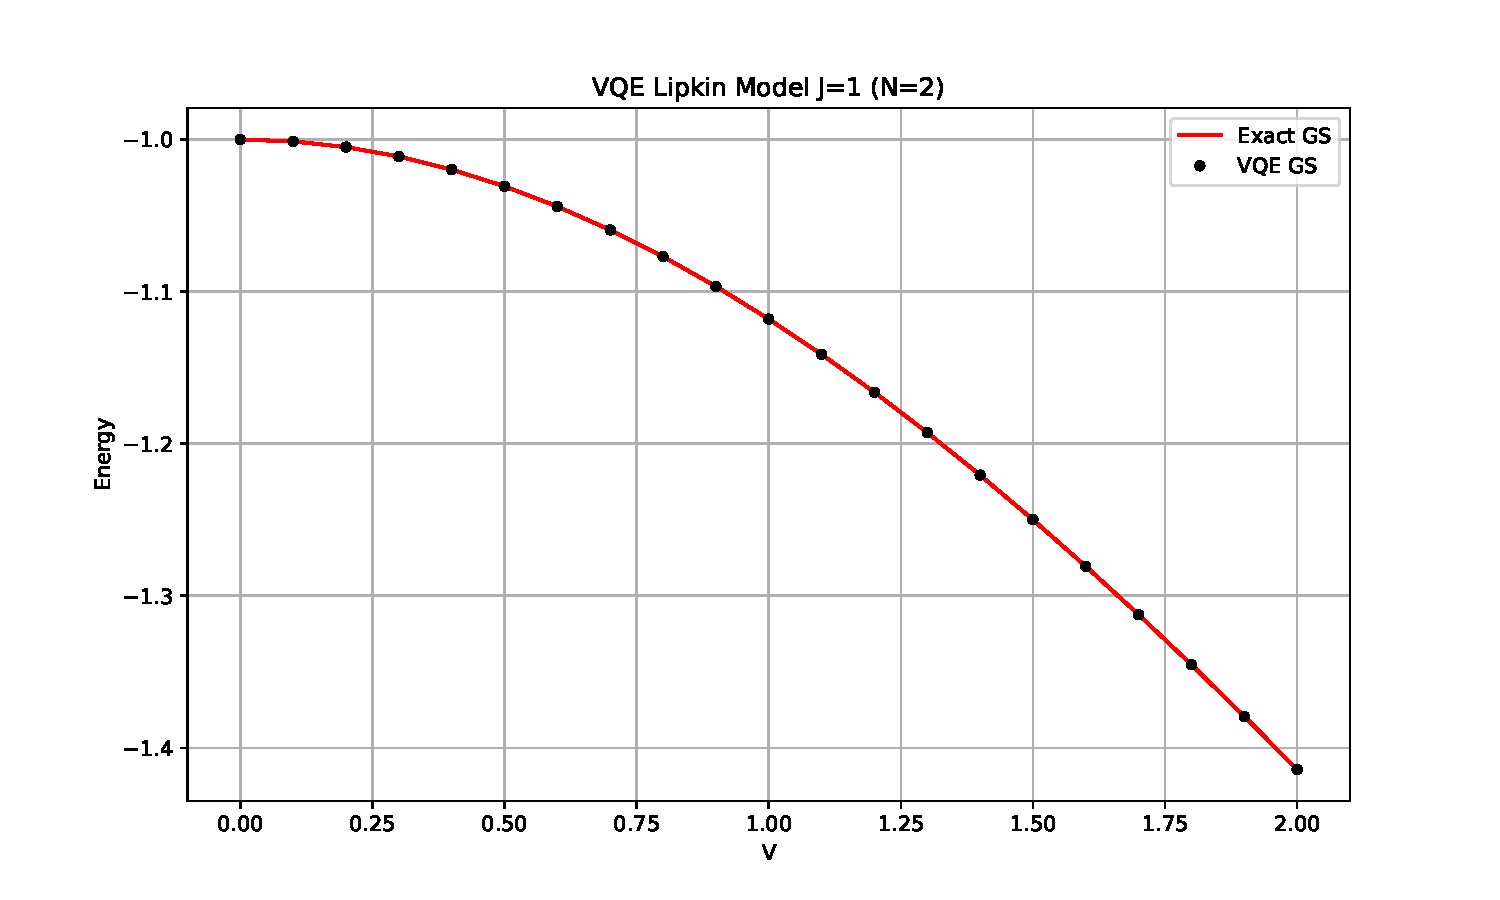
\includegraphics[width=0.55\linewidth]{figures/part-g_vqe_j1.pdf}
    \caption{VQE optimization landscape under variation of $J_1$ (Part G).}
    \label{fig:partg_vqe_j1}
\end{figure}